\section{Durchführung}
Zu Beginn wird die Leelaufspannung mit Hilfe eines Spannungsmessers bestimmt sowie deren Eigenwiderstand.
In Abbildung (\ref{abb:2}) werden aus unterschiedlichen Spannungsformen (in diesem Fall Gleich-,Rechteck- und Sinusspannung)
die Spannungswerte sowie Stromwerte notiert.
\begin{figure}[H]
  \centering
  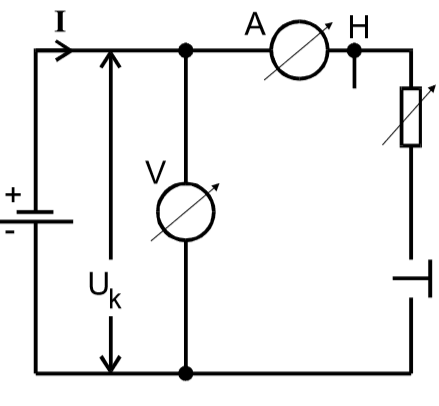
\includegraphics[width= 10 cm , height=7 cm]{Bild2.png}
  \caption{Stromkreis zu Bestimmung von $U_0$ und $R_i$ \cite{1}}
  \label{abb:2}
\end{figure}
In Abbildung (\ref{abb:3}) ist nun eine Gegenspannung angeschlossen. Dies bewirkt, dass sich der Stromfluß
ändert.
\begin{figure}[H]
  \centering
  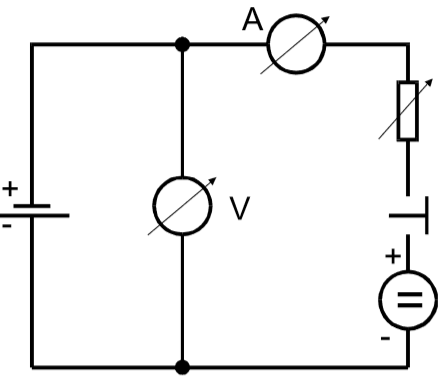
\includegraphics[width=10 cm, height= 7 cm]{Bild3.png}
  \caption{Stromkreis zu Bestimmung von $U_0$ und $R_i$ \cite{1}}
  \label{abb:3}
\end{figure}
